\documentclass[1p]{elsarticle_modified}
%\bibliographystyle{elsarticle-num}

%\usepackage[colorlinks]{hyperref}
%\usepackage{abbrmath_seonhwa} %\Abb, \Ascr, \Acal ,\Abf, \Afrak
\usepackage{amsfonts}
\usepackage{amssymb}
\usepackage{amsmath}
\usepackage{amsthm}
\usepackage{scalefnt}
\usepackage{amsbsy}
\usepackage{kotex}
\usepackage{caption}
\usepackage{subfig}
\usepackage{color}
\usepackage{graphicx}
\usepackage{xcolor} %% white, black, red, green, blue, cyan, magenta, yellow
\usepackage{float}
\usepackage{setspace}
\usepackage{hyperref}

\usepackage{tikz}
\usetikzlibrary{arrows}

\usepackage{multirow}
\usepackage{array} % fixed length table
\usepackage{hhline}

%%%%%%%%%%%%%%%%%%%%%
\makeatletter
\renewcommand*\env@matrix[1][\arraystretch]{%
	\edef\arraystretch{#1}%
	\hskip -\arraycolsep
	\let\@ifnextchar\new@ifnextchar
	\array{*\c@MaxMatrixCols c}}
\makeatother %https://tex.stackexchange.com/questions/14071/how-can-i-increase-the-line-spacing-in-a-matrix
%%%%%%%%%%%%%%%

\usepackage[normalem]{ulem}

\newcommand{\msout}[1]{\ifmmode\text{\sout{\ensuremath{#1}}}\else\sout{#1}\fi}
%SOURCE: \msout is \stkout macro in https://tex.stackexchange.com/questions/20609/strikeout-in-math-mode

\newcommand{\cancel}[1]{
	\ifmmode
	{\color{red}\msout{#1}}
	\else
	{\color{red}\sout{#1}}
	\fi
}

\newcommand{\add}[1]{
	{\color{blue}\uwave{#1}}
}

\newcommand{\replace}[2]{
	\ifmmode
	{\color{red}\msout{#1}}{\color{blue}\uwave{#2}}
	\else
	{\color{red}\sout{#1}}{\color{blue}\uwave{#2}}
	\fi
}

\newcommand{\Sol}{\mathcal{S}} %segment
\newcommand{\D}{D} %diagram
\newcommand{\A}{\mathcal{A}} %arc


%%%%%%%%%%%%%%%%%%%%%%%%%%%%%5 test

\def\sl{\operatorname{\textup{SL}}(2,\Cbb)}
\def\psl{\operatorname{\textup{PSL}}(2,\Cbb)}
\def\quan{\mkern 1mu \triangleright \mkern 1mu}

\theoremstyle{definition}
\newtheorem{thm}{Theorem}[section]
\newtheorem{prop}[thm]{Proposition}
\newtheorem{lem}[thm]{Lemma}
\newtheorem{ques}[thm]{Question}
\newtheorem{cor}[thm]{Corollary}
\newtheorem{defn}[thm]{Definition}
\newtheorem{exam}[thm]{Example}
\newtheorem{rmk}[thm]{Remark}
\newtheorem{alg}[thm]{Algorithm}

\newcommand{\I}{\sqrt{-1}}
\begin{document}

%\begin{frontmatter}
%
%\title{Boundary parabolic representations of knots up to 8 crossings}
%
%%% Group authors per affiliation:
%\author{Yunhi Cho} 
%\address{Department of Mathematics, University of Seoul, Seoul, Korea}
%\ead{yhcho@uos.ac.kr}
%
%
%\author{Seonhwa Kim} %\fnref{s_kim}}
%\address{Center for Geometry and Physics, Institute for Basic Science, Pohang, 37673, Korea}
%\ead{ryeona17@ibs.re.kr}
%
%\author{Hyuk Kim}
%\address{Department of Mathematical Sciences, Seoul National University, Seoul 08826, Korea}
%\ead{hyukkim@snu.ac.kr}
%
%\author{Seokbeom Yoon}
%\address{Department of Mathematical Sciences, Seoul National University, Seoul, 08826,  Korea}
%\ead{sbyoon15@snu.ac.kr}
%
%\begin{abstract}
%We find all boundary parabolic representation of knots up to 8 crossings.
%
%\end{abstract}
%\begin{keyword}
%    \MSC[2010] 57M25 
%\end{keyword}
%
%\end{frontmatter}

%\linenumbers
%\tableofcontents
%
\newcommand\colored[1]{\textcolor{white}{\rule[-0.35ex]{0.8em}{1.4ex}}\kern-0.8em\color{red} #1}%
%\newcommand\colored[1]{\textcolor{white}{ #1}\kern-2.17ex	\textcolor{white}{ #1}\kern-1.81ex	\textcolor{white}{ #1}\kern-2.15ex\color{red}#1	}

{\Large $\underline{12n_{0211}~(K12n_{0211})}$}

\setlength{\tabcolsep}{10pt}
\renewcommand{\arraystretch}{1.6}
\vspace{1cm}\begin{tabular}{m{100pt}>{\centering\arraybackslash}m{274pt}}
\multirow{5}{120pt}{
	\centering
	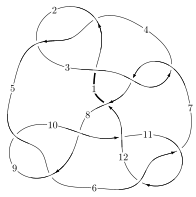
\includegraphics[width=112pt]{../../../GIT/diagram.site/Diagrams/png/2300_12n_0211.png}\\
\ \ \ A knot diagram\footnotemark}&
\allowdisplaybreaks
\textbf{Linearized knot diagam} \\
\cline{2-2}
 &
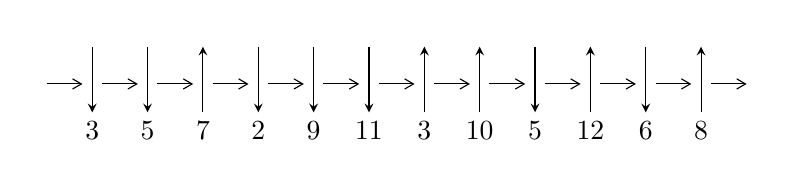
\begin{tikzpicture}[x=20pt, y=17pt]
	% nodes
	\node (C0) at (0, 0) {};
	\node (C1) at (1, 0) {};
	\node (C1U) at (1, +1) {};
	\node (C1D) at (1, -1) {3};

	\node (C2) at (2, 0) {};
	\node (C2U) at (2, +1) {};
	\node (C2D) at (2, -1) {5};

	\node (C3) at (3, 0) {};
	\node (C3U) at (3, +1) {};
	\node (C3D) at (3, -1) {7};

	\node (C4) at (4, 0) {};
	\node (C4U) at (4, +1) {};
	\node (C4D) at (4, -1) {2};

	\node (C5) at (5, 0) {};
	\node (C5U) at (5, +1) {};
	\node (C5D) at (5, -1) {9};

	\node (C6) at (6, 0) {};
	\node (C6U) at (6, +1) {};
	\node (C6D) at (6, -1) {11};

	\node (C7) at (7, 0) {};
	\node (C7U) at (7, +1) {};
	\node (C7D) at (7, -1) {3};

	\node (C8) at (8, 0) {};
	\node (C8U) at (8, +1) {};
	\node (C8D) at (8, -1) {10};

	\node (C9) at (9, 0) {};
	\node (C9U) at (9, +1) {};
	\node (C9D) at (9, -1) {5};

	\node (C10) at (10, 0) {};
	\node (C10U) at (10, +1) {};
	\node (C10D) at (10, -1) {12};

	\node (C11) at (11, 0) {};
	\node (C11U) at (11, +1) {};
	\node (C11D) at (11, -1) {6};

	\node (C12) at (12, 0) {};
	\node (C12U) at (12, +1) {};
	\node (C12D) at (12, -1) {8};
	\node (C13) at (13, 0) {};

	% arrows
	\draw[->,>={angle 60}]
	(C0) edge (C1) (C1) edge (C2) (C2) edge (C3) (C3) edge (C4) (C4) edge (C5) (C5) edge (C6) (C6) edge (C7) (C7) edge (C8) (C8) edge (C9) (C9) edge (C10) (C10) edge (C11) (C11) edge (C12) (C12) edge (C13) ;	\draw[->,>=stealth]
	(C1U) edge (C1D) (C2U) edge (C2D) (C3D) edge (C3U) (C4U) edge (C4D) (C5U) edge (C5D) (C6U) edge (C6D) (C7D) edge (C7U) (C8D) edge (C8U) (C9U) edge (C9D) (C10D) edge (C10U) (C11U) edge (C11D) (C12D) edge (C12U) ;
	\end{tikzpicture} \\
\hhline{~~} \\& 
\textbf{Solving Sequence} \\ \cline{2-2} 
 &
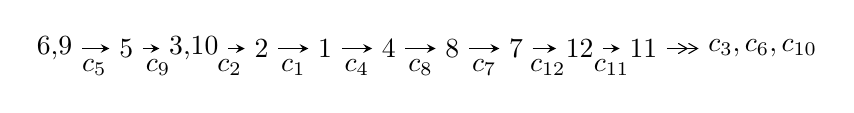
\begin{tikzpicture}[x=23pt, y=7pt]
	% node
	\node (A0) at (-1/8, 0) {6,9};
	\node (A1) at (1, 0) {5};
	\node (A2) at (33/16, 0) {3,10};
	\node (A3) at (25/8, 0) {2};
	\node (A4) at (33/8, 0) {1};
	\node (A5) at (41/8, 0) {4};
	\node (A6) at (49/8, 0) {8};
	\node (A7) at (57/8, 0) {7};
	\node (A8) at (65/8, 0) {12};
	\node (A9) at (73/8, 0) {11};
	\node (C1) at (1/2, -1) {$c_{5}$};
	\node (C2) at (3/2, -1) {$c_{9}$};
	\node (C3) at (21/8, -1) {$c_{2}$};
	\node (C4) at (29/8, -1) {$c_{1}$};
	\node (C5) at (37/8, -1) {$c_{4}$};
	\node (C6) at (45/8, -1) {$c_{8}$};
	\node (C7) at (53/8, -1) {$c_{7}$};
	\node (C8) at (61/8, -1) {$c_{12}$};
	\node (C9) at (69/8, -1) {$c_{11}$};
	\node (A10) at (11, 0) {$c_{3},c_{6},c_{10}$};

	% edge
	\draw[->,>=stealth]	
	(A0) edge (A1) (A1) edge (A2) (A2) edge (A3) (A3) edge (A4) (A4) edge (A5) (A5) edge (A6) (A6) edge (A7) (A7) edge (A8) (A8) edge (A9) ;
	\draw[->>,>={angle 60}]	
	(A9) edge (A10);
\end{tikzpicture} \\ 

\end{tabular} \\

\footnotetext{
The image of knot diagram is generated by the software ``\textbf{Draw programme}" developed by Andrew Bartholomew(\url{http://www.layer8.co.uk/maths/draw/index.htm\#Running-draw}), where we modified some parts for our purpose(\url{https://github.com/CATsTAILs/LinksPainter}).
}\phantom \\ \newline 
\centering \textbf{Ideals for irreducible components\footnotemark of $X_{\text{par}}$} 
 
\begin{align*}
I^u_{1}&=\langle 
13 u^{16}+9 u^{15}+\cdots+32 b+15,\;21 u^{16}-15 u^{15}+\cdots+32 a-41,\\
\phantom{I^u_{1}}&\phantom{= \langle  }u^{17}+3 u^{15}+2 u^{14}+9 u^{13}+4 u^{12}+15 u^{11}+9 u^{10}+23 u^9+6 u^8+23 u^7+5 u^6+19 u^5-3 u^4+11 u^3+1\rangle \\
I^u_{2}&=\langle 
- u^3+u^2+2 b+1,\;- u^3- u^2+2 a-1,\;u^4+u^2- u+1\rangle \\
I^u_{3}&=\langle 
-33675480 u^{21}+230853871 u^{20}+\cdots+427516113 b+1988747145,\\
\phantom{I^u_{3}}&\phantom{= \langle  }-330664297 u^{21}+1163900912 u^{20}+\cdots+1282548339 a+9330160065,\\
\phantom{I^u_{3}}&\phantom{= \langle  }u^{22}-2 u^{21}+\cdots-12 u+9\rangle \\
I^u_{4}&=\langle 
u^5+u^4+u^3+2 u^2+b+u+1,\;u^5+u^4+u^3+u^2+a+u,\;u^6+u^5+2 u^4+2 u^3+2 u^2+2 u+1\rangle \\
I^u_{5}&=\langle 
a u+5 b-3 a+u-3,\;a^2+a u+5 u-4,\;u^2+1\rangle \\
\\
\end{align*}
\raggedright * 5 irreducible components of $\dim_{\mathbb{C}}=0$, with total 53 representations.\\
\footnotetext{All coefficients of polynomials are rational numbers. But the coefficients are sometimes approximated in decimal forms when there is not enough margin.}
\newpage
\renewcommand{\arraystretch}{1}
\centering \section*{I. $I^u_{1}= \langle 13 u^{16}+9 u^{15}+\cdots+32 b+15,\;21 u^{16}-15 u^{15}+\cdots+32 a-41,\;u^{17}+3 u^{15}+\cdots+11 u^3+1 \rangle$}
\flushleft \textbf{(i) Arc colorings}\\
\begin{tabular}{m{7pt} m{180pt} m{7pt} m{180pt} }
\flushright $a_{6}=$&$\begin{pmatrix}1\\0\end{pmatrix}$ \\
\flushright $a_{9}=$&$\begin{pmatrix}0\\u\end{pmatrix}$ \\
\flushright $a_{5}=$&$\begin{pmatrix}1\\- u^2\end{pmatrix}$ \\
\flushright $a_{3}=$&$\begin{pmatrix}-0.656250 u^{16}+0.468750 u^{15}+\cdots+2.90625 u+1.28125\\-0.406250 u^{16}-0.281250 u^{15}+\cdots-0.343750 u-0.468750\end{pmatrix}$ \\
\flushright $a_{10}=$&$\begin{pmatrix}- u\\u^3+u\end{pmatrix}$ \\
\flushright $a_{2}=$&$\begin{pmatrix}-0.468750 u^{16}+0.406250 u^{15}+\cdots+3.21875 u+0.343750\\-0.0937500 u^{16}-0.218750 u^{15}+\cdots-0.156250 u-0.531250\end{pmatrix}$ \\
\flushright $a_{1}=$&$\begin{pmatrix}\frac{1}{2} u^{16}+u^{14}+\cdots-\frac{5}{2} u^3+\frac{5}{2} u\\\frac{1}{4} u^{16}+\frac{1}{2} u^{14}+\cdots-\frac{9}{4} u^3-\frac{3}{4} u\end{pmatrix}$ \\
\flushright $a_{4}=$&$\begin{pmatrix}-0.281250 u^{16}+0.0937500 u^{15}+\cdots+2.53125 u+0.156250\\-0.531250 u^{16}+0.0937500 u^{15}+\cdots+0.281250 u+0.156250\end{pmatrix}$ \\
\flushright $a_{8}=$&$\begin{pmatrix}- u^3\\u^5+u^3+u\end{pmatrix}$ \\
\flushright $a_{7}=$&$\begin{pmatrix}\frac{1}{4} u^{15}+\frac{1}{2} u^{13}+\cdots-\frac{5}{4} u^2+\frac{5}{4}\\u^2\end{pmatrix}$ \\
\flushright $a_{12}=$&$\begin{pmatrix}\frac{1}{4} u^{16}+\frac{1}{2} u^{14}+\cdots-\frac{9}{4} u^3+\frac{9}{4} u\\- u\end{pmatrix}$ \\
\flushright $a_{11}=$&$\begin{pmatrix}\frac{1}{4} u^{16}+\frac{1}{2} u^{14}+\cdots-\frac{9}{4} u^3+\frac{5}{4} u\\- u\end{pmatrix}$\\&\end{tabular}
\flushleft \textbf{(ii) Obstruction class $= -1$}\\~\\
\flushleft \textbf{(iii) Cusp Shapes $= \frac{25}{64} u^{16}+\frac{61}{64} u^{15}+\cdots+\frac{639}{64} u-\frac{133}{64}$}\\~\\
\newpage\renewcommand{\arraystretch}{1}
\flushleft \textbf{(iv) u-Polynomials at the component}\newline \\
\begin{tabular}{m{50pt}|m{274pt}}
Crossings & \hspace{64pt}u-Polynomials at each crossing \\
\hline $$\begin{aligned}c_{1}\end{aligned}$$&$\begin{aligned}
&u^{17}+25 u^{16}+\cdots-31 u+16
\end{aligned}$\\
\hline $$\begin{aligned}c_{2},c_{4}\end{aligned}$$&$\begin{aligned}
&u^{17}-5 u^{16}+\cdots- u+4
\end{aligned}$\\
\hline $$\begin{aligned}c_{3},c_{7}\end{aligned}$$&$\begin{aligned}
&u^{17}-3 u^{16}+\cdots+176 u+64
\end{aligned}$\\
\hline $$\begin{aligned}c_{5},c_{6},c_{9}\\c_{11}\end{aligned}$$&$\begin{aligned}
&u^{17}+3 u^{15}+\cdots+11 u^3-1
\end{aligned}$\\
\hline $$\begin{aligned}c_{8},c_{10}\end{aligned}$$&$\begin{aligned}
&u^{17}-6 u^{16}+\cdots-6 u^2+1
\end{aligned}$\\
\hline $$\begin{aligned}c_{12}\end{aligned}$$&$\begin{aligned}
&u^{17}+19 u^{15}+\cdots-5 u^2+4
\end{aligned}$\\
\hline
\end{tabular}\\~\\
\newpage\renewcommand{\arraystretch}{1}
\flushleft \textbf{(v) Riley Polynomials at the component}\newline \\
\begin{tabular}{m{50pt}|m{274pt}}
Crossings & \hspace{64pt}Riley Polynomials at each crossing \\
\hline $$\begin{aligned}c_{1}\end{aligned}$$&$\begin{aligned}
&y^{17}-61 y^{16}+\cdots-15103 y-256
\end{aligned}$\\
\hline $$\begin{aligned}c_{2},c_{4}\end{aligned}$$&$\begin{aligned}
&y^{17}-25 y^{16}+\cdots-31 y-16
\end{aligned}$\\
\hline $$\begin{aligned}c_{3},c_{7}\end{aligned}$$&$\begin{aligned}
&y^{17}+27 y^{16}+\cdots+4352 y-4096
\end{aligned}$\\
\hline $$\begin{aligned}c_{5},c_{6},c_{9}\\c_{11}\end{aligned}$$&$\begin{aligned}
&y^{17}+6 y^{16}+\cdots+6 y^2-1
\end{aligned}$\\
\hline $$\begin{aligned}c_{8},c_{10}\end{aligned}$$&$\begin{aligned}
&y^{17}+18 y^{16}+\cdots+12 y-1
\end{aligned}$\\
\hline $$\begin{aligned}c_{12}\end{aligned}$$&$\begin{aligned}
&y^{17}+38 y^{16}+\cdots+40 y-16
\end{aligned}$\\
\hline
\end{tabular}\\~\\
\newpage\flushleft \textbf{(vi) Complex Volumes and Cusp Shapes}
$$\begin{array}{c|c|c}  
\text{Solutions to }I^u_{1}& \I (\text{vol} + \sqrt{-1}CS) & \text{Cusp shape}\\
 \hline 
\begin{aligned}
u &= \phantom{-}0.609453 + 0.805159 I \\
a &= \phantom{-}0.854862 - 0.986654 I \\
b &= -0.766890 - 0.457544 I\end{aligned}
 & -0.52072 - 2.33309 I & -2.02167 + 3.26936 I \\ \hline\begin{aligned}
u &= \phantom{-}0.609453 - 0.805159 I \\
a &= \phantom{-}0.854862 + 0.986654 I \\
b &= -0.766890 + 0.457544 I\end{aligned}
 & -0.52072 + 2.33309 I & -2.02167 - 3.26936 I \\ \hline\begin{aligned}
u &= \phantom{-}0.230202 + 0.870288 I \\
a &= -2.22993 - 0.26645 I \\
b &= -0.119488 + 0.657240 I\end{aligned}
 & -6.16563 - 1.02177 I & -6.84477 + 7.08191 I \\ \hline\begin{aligned}
u &= \phantom{-}0.230202 - 0.870288 I \\
a &= -2.22993 + 0.26645 I \\
b &= -0.119488 - 0.657240 I\end{aligned}
 & -6.16563 + 1.02177 I & -6.84477 - 7.08191 I \\ \hline\begin{aligned}
u &= -0.773626 + 0.937847 I \\
a &= \phantom{-}0.606886 - 0.071826 I \\
b &= -1.190660 + 0.370945 I\end{aligned}
 & -4.38989 + 4.09446 I & -5.30008 - 4.36784 I \\ \hline\begin{aligned}
u &= -0.773626 - 0.937847 I \\
a &= \phantom{-}0.606886 + 0.071826 I \\
b &= -1.190660 - 0.370945 I\end{aligned}
 & -4.38989 - 4.09446 I & -5.30008 + 4.36784 I \\ \hline\begin{aligned}
u &= -1.050610 + 0.636095 I \\
a &= -0.407370 + 0.267779 I \\
b &= \phantom{-}1.93722 - 0.60149 I\end{aligned}
 & -17.5984 - 0.0758 I & -7.31042 - 1.57550 I \\ \hline\begin{aligned}
u &= -1.050610 - 0.636095 I \\
a &= -0.407370 - 0.267779 I \\
b &= \phantom{-}1.93722 + 0.60149 I\end{aligned}
 & -17.5984 + 0.0758 I & -7.31042 + 1.57550 I \\ \hline\begin{aligned}
u &= -0.576669 + 1.098490 I \\
a &= -0.263264 - 0.069567 I \\
b &= \phantom{-}0.341659 - 0.129445 I\end{aligned}
 & \phantom{-}1.86747 + 7.21175 I & \phantom{-}3.72852 - 5.27936 I \\ \hline\begin{aligned}
u &= -0.576669 - 1.098490 I \\
a &= -0.263264 + 0.069567 I \\
b &= \phantom{-}0.341659 + 0.129445 I\end{aligned}
 & \phantom{-}1.86747 - 7.21175 I & \phantom{-}3.72852 + 5.27936 I\\
 \hline 
 \end{array}$$\newpage$$\begin{array}{c|c|c}  
\text{Solutions to }I^u_{1}& \I (\text{vol} + \sqrt{-1}CS) & \text{Cusp shape}\\
 \hline 
\begin{aligned}
u &= \phantom{-}0.743234 + 1.053510 I \\
a &= -0.04444 + 2.04366 I \\
b &= \phantom{-}2.07902 + 0.33370 I\end{aligned}
 & -3.55752 - 7.80542 I & -4.29962 + 6.17985 I \\ \hline\begin{aligned}
u &= \phantom{-}0.743234 - 1.053510 I \\
a &= -0.04444 - 2.04366 I \\
b &= \phantom{-}2.07902 - 0.33370 I\end{aligned}
 & -3.55752 + 7.80542 I & -4.29962 - 6.17985 I \\ \hline\begin{aligned}
u &= \phantom{-}0.71574 + 1.23305 I \\
a &= -0.99869 - 1.97392 I \\
b &= -2.63254 + 0.11082 I\end{aligned}
 & -13.5091 - 13.2681 I & -3.78464 + 6.49717 I \\ \hline\begin{aligned}
u &= \phantom{-}0.71574 - 1.23305 I \\
a &= -0.99869 + 1.97392 I \\
b &= -2.63254 - 0.11082 I\end{aligned}
 & -13.5091 + 13.2681 I & -3.78464 - 6.49717 I \\ \hline\begin{aligned}
u &= \phantom{-}0.302591 + 0.411010 I \\
a &= \phantom{-}0.856584 + 0.998116 I \\
b &= \phantom{-}0.086217 - 0.461654 I\end{aligned}
 & -0.250655 - 1.078620 I & -3.32954 + 6.69723 I \\ \hline\begin{aligned}
u &= \phantom{-}0.302591 - 0.411010 I \\
a &= \phantom{-}0.856584 - 0.998116 I \\
b &= \phantom{-}0.086217 + 0.461654 I\end{aligned}
 & -0.250655 + 1.078620 I & -3.32954 - 6.69723 I \\ \hline\begin{aligned}
u &= -0.400636\phantom{ +0.000000I} \\
a &= -1.24927\phantom{ +0.000000I} \\
b &= -0.969091\phantom{ +0.000000I}\end{aligned}
 & -2.22247\phantom{ +0.000000I} & -4.42560\phantom{ +0.000000I}\\
 \hline 
 \end{array}$$\newpage\newpage\renewcommand{\arraystretch}{1}
\centering \section*{II. $I^u_{2}= \langle - u^3+u^2+2 b+1,\;- u^3- u^2+2 a-1,\;u^4+u^2- u+1 \rangle$}
\flushleft \textbf{(i) Arc colorings}\\
\begin{tabular}{m{7pt} m{180pt} m{7pt} m{180pt} }
\flushright $a_{6}=$&$\begin{pmatrix}1\\0\end{pmatrix}$ \\
\flushright $a_{9}=$&$\begin{pmatrix}0\\u\end{pmatrix}$ \\
\flushright $a_{5}=$&$\begin{pmatrix}1\\- u^2\end{pmatrix}$ \\
\flushright $a_{3}=$&$\begin{pmatrix}\frac{1}{2} u^3+\frac{1}{2} u^2+\frac{1}{2}\\\frac{1}{2} u^3-\frac{1}{2} u^2-\frac{1}{2}\end{pmatrix}$ \\
\flushright $a_{10}=$&$\begin{pmatrix}- u\\u^3+u\end{pmatrix}$ \\
\flushright $a_{2}=$&$\begin{pmatrix}\frac{1}{2} u^3+\frac{1}{2} u^2-\frac{1}{2}\\\frac{1}{2} u^3+\frac{1}{2} u^2-\frac{1}{2}\end{pmatrix}$ \\
\flushright $a_{1}=$&$\begin{pmatrix}-1\\u^2\end{pmatrix}$ \\
\flushright $a_{4}=$&$\begin{pmatrix}\frac{1}{2} u^3+\frac{1}{2} u^2+\frac{1}{2}\\\frac{1}{2} u^3-\frac{1}{2} u^2-\frac{1}{2}\end{pmatrix}$ \\
\flushright $a_{8}=$&$\begin{pmatrix}- u^3\\u^2\end{pmatrix}$ \\
\flushright $a_{7}=$&$\begin{pmatrix}- u^3\\u^2\end{pmatrix}$ \\
\flushright $a_{12}=$&$\begin{pmatrix}u^3- u^2-1\\u\end{pmatrix}$ \\
\flushright $a_{11}=$&$\begin{pmatrix}u^3- u^2+u-1\\u\end{pmatrix}$\\&\end{tabular}
\flushleft \textbf{(ii) Obstruction class $= 1$}\\~\\
\flushleft \textbf{(iii) Cusp Shapes $= \frac{11}{4} u^3+\frac{21}{4} u^2-\frac{1}{2} u-\frac{17}{4}$}\\~\\
\newpage\renewcommand{\arraystretch}{1}
\flushleft \textbf{(iv) u-Polynomials at the component}\newline \\
\begin{tabular}{m{50pt}|m{274pt}}
Crossings & \hspace{64pt}u-Polynomials at each crossing \\
\hline $$\begin{aligned}c_{1},c_{2}\end{aligned}$$&$\begin{aligned}
&(u-1)^4
\end{aligned}$\\
\hline $$\begin{aligned}c_{3},c_{7}\end{aligned}$$&$\begin{aligned}
&u^4
\end{aligned}$\\
\hline $$\begin{aligned}c_{4}\end{aligned}$$&$\begin{aligned}
&(u+1)^4
\end{aligned}$\\
\hline $$\begin{aligned}c_{5},c_{6}\end{aligned}$$&$\begin{aligned}
&u^4+u^2- u+1
\end{aligned}$\\
\hline $$\begin{aligned}c_{8},c_{10}\end{aligned}$$&$\begin{aligned}
&u^4+2 u^3+3 u^2+u+1
\end{aligned}$\\
\hline $$\begin{aligned}c_{9},c_{11}\end{aligned}$$&$\begin{aligned}
&u^4+u^2+u+1
\end{aligned}$\\
\hline $$\begin{aligned}c_{12}\end{aligned}$$&$\begin{aligned}
&u^4+3 u^3+4 u^2+3 u+2
\end{aligned}$\\
\hline
\end{tabular}\\~\\
\newpage\renewcommand{\arraystretch}{1}
\flushleft \textbf{(v) Riley Polynomials at the component}\newline \\
\begin{tabular}{m{50pt}|m{274pt}}
Crossings & \hspace{64pt}Riley Polynomials at each crossing \\
\hline $$\begin{aligned}c_{1},c_{2},c_{4}\end{aligned}$$&$\begin{aligned}
&(y-1)^4
\end{aligned}$\\
\hline $$\begin{aligned}c_{3},c_{7}\end{aligned}$$&$\begin{aligned}
&y^4
\end{aligned}$\\
\hline $$\begin{aligned}c_{5},c_{6},c_{9}\\c_{11}\end{aligned}$$&$\begin{aligned}
&y^4+2 y^3+3 y^2+y+1
\end{aligned}$\\
\hline $$\begin{aligned}c_{8},c_{10}\end{aligned}$$&$\begin{aligned}
&y^4+2 y^3+7 y^2+5 y+1
\end{aligned}$\\
\hline $$\begin{aligned}c_{12}\end{aligned}$$&$\begin{aligned}
&y^4- y^3+2 y^2+7 y+4
\end{aligned}$\\
\hline
\end{tabular}\\~\\
\newpage\flushleft \textbf{(vi) Complex Volumes and Cusp Shapes}
$$\begin{array}{c|c|c}  
\text{Solutions to }I^u_{2}& \I (\text{vol} + \sqrt{-1}CS) & \text{Cusp shape}\\
 \hline 
\begin{aligned}
u &= \phantom{-}0.547424 + 0.585652 I \\
a &= \phantom{-}0.278726 + 0.483420 I \\
b &= -0.677958 - 0.157780 I\end{aligned}
 & -2.62503 - 1.39709 I & -5.84901 + 3.96898 I \\ \hline\begin{aligned}
u &= \phantom{-}0.547424 - 0.585652 I \\
a &= \phantom{-}0.278726 - 0.483420 I \\
b &= -0.677958 + 0.157780 I\end{aligned}
 & -2.62503 + 1.39709 I & -5.84901 - 3.96898 I \\ \hline\begin{aligned}
u &= -0.547424 + 1.120870 I \\
a &= \phantom{-}0.971274 - 0.813859 I \\
b &= \phantom{-}0.927958 + 0.413327 I\end{aligned}
 & \phantom{-}0.98010 + 7.64338 I & -3.77599 - 8.10462 I \\ \hline\begin{aligned}
u &= -0.547424 - 1.120870 I \\
a &= \phantom{-}0.971274 + 0.813859 I \\
b &= \phantom{-}0.927958 - 0.413327 I\end{aligned}
 & \phantom{-}0.98010 - 7.64338 I & -3.77599 + 8.10462 I\\
 \hline 
 \end{array}$$\newpage\newpage\renewcommand{\arraystretch}{1}
\centering \section*{III. $I^u_{3}= \langle -3.37\times10^{7} u^{21}+2.31\times10^{8} u^{20}+\cdots+4.28\times10^{8} b+1.99\times10^{9},\;-3.31\times10^{8} u^{21}+1.16\times10^{9} u^{20}+\cdots+1.28\times10^{9} a+9.33\times10^{9},\;u^{22}-2 u^{21}+\cdots-12 u+9 \rangle$}
\flushleft \textbf{(i) Arc colorings}\\
\begin{tabular}{m{7pt} m{180pt} m{7pt} m{180pt} }
\flushright $a_{6}=$&$\begin{pmatrix}1\\0\end{pmatrix}$ \\
\flushright $a_{9}=$&$\begin{pmatrix}0\\u\end{pmatrix}$ \\
\flushright $a_{5}=$&$\begin{pmatrix}1\\- u^2\end{pmatrix}$ \\
\flushright $a_{3}=$&$\begin{pmatrix}0.257818 u^{21}-0.907491 u^{20}+\cdots+8.27519 u-7.27470\\0.0787701 u^{21}-0.539989 u^{20}+\cdots+5.17053 u-4.65186\end{pmatrix}$ \\
\flushright $a_{10}=$&$\begin{pmatrix}- u\\u^3+u\end{pmatrix}$ \\
\flushright $a_{2}=$&$\begin{pmatrix}0.0569753 u^{21}-0.732717 u^{20}+\cdots+6.42310 u-8.39988\\0.147735 u^{21}-0.732052 u^{20}+\cdots+6.08589 u-6.69407\end{pmatrix}$ \\
\flushright $a_{1}=$&$\begin{pmatrix}-0.113449 u^{21}-0.132459 u^{20}+\cdots+2.54918 u-1.84329\\0.183373 u^{21}-0.457606 u^{20}+\cdots+4.47394 u-2.89558\end{pmatrix}$ \\
\flushright $a_{4}=$&$\begin{pmatrix}-0.325326 u^{21}+0.184523 u^{20}+\cdots+0.502711 u-2.87359\\-0.383495 u^{21}+0.177086 u^{20}+\cdots-0.310468 u-2.63640\end{pmatrix}$ \\
\flushright $a_{8}=$&$\begin{pmatrix}- u^3\\u^5+u^3+u\end{pmatrix}$ \\
\flushright $a_{7}=$&$\begin{pmatrix}-0.264604 u^{21}+0.445061 u^{20}+\cdots-3.11735 u-0.705220\\-0.121794 u^{21}+0.190645 u^{20}+\cdots-0.910828 u-1.28085\end{pmatrix}$ \\
\flushright $a_{12}=$&$\begin{pmatrix}\frac{1}{9} u^{21}-\frac{2}{9} u^{20}+\cdots+\frac{32}{9} u-\frac{4}{3}\\0.0312057 u^{21}-0.184205 u^{20}+\cdots+2.13810 u-1.28530\end{pmatrix}$ \\
\flushright $a_{11}=$&$\begin{pmatrix}0.142317 u^{21}-0.406427 u^{20}+\cdots+5.69365 u-2.61863\\0.0312057 u^{21}-0.184205 u^{20}+\cdots+2.13810 u-1.28530\end{pmatrix}$\\&\end{tabular}
\flushleft \textbf{(ii) Obstruction class $= -1$}\\~\\
\flushleft \textbf{(iii) Cusp Shapes $= -\frac{51496451}{142505371} u^{21}+\frac{36892662}{142505371} u^{20}+\cdots+\frac{723246262}{142505371} u-\frac{1135221198}{142505371}$}\\~\\
\newpage\renewcommand{\arraystretch}{1}
\flushleft \textbf{(iv) u-Polynomials at the component}\newline \\
\begin{tabular}{m{50pt}|m{274pt}}
Crossings & \hspace{64pt}u-Polynomials at each crossing \\
\hline $$\begin{aligned}c_{1}\end{aligned}$$&$\begin{aligned}
&(u^{11}+18 u^{10}+\cdots+31 u+1)^{2}
\end{aligned}$\\
\hline $$\begin{aligned}c_{2},c_{4}\end{aligned}$$&$\begin{aligned}
&(u^{11}-4 u^{10}- u^9+17 u^8+u^7-40 u^6+3 u^5+37 u^4-3 u^3-9 u^2+7 u-1)^{2}
\end{aligned}$\\
\hline $$\begin{aligned}c_{3},c_{7}\end{aligned}$$&$\begin{aligned}
&(u^{11}+u^{10}+\cdots-4 u+8)^{2}
\end{aligned}$\\
\hline $$\begin{aligned}c_{5},c_{6},c_{9}\\c_{11}\end{aligned}$$&$\begin{aligned}
&u^{22}+2 u^{21}+\cdots+12 u+9
\end{aligned}$\\
\hline $$\begin{aligned}c_{8},c_{10}\end{aligned}$$&$\begin{aligned}
&u^{22}-10 u^{21}+\cdots-432 u+81
\end{aligned}$\\
\hline $$\begin{aligned}c_{12}\end{aligned}$$&$\begin{aligned}
&(u^{11}+12 u^9+36 u^7+2 u^6+2 u^5+13 u^4+13 u^3+u^2+1)^2
\end{aligned}$\\
\hline
\end{tabular}\\~\\
\newpage\renewcommand{\arraystretch}{1}
\flushleft \textbf{(v) Riley Polynomials at the component}\newline \\
\begin{tabular}{m{50pt}|m{274pt}}
Crossings & \hspace{64pt}Riley Polynomials at each crossing \\
\hline $$\begin{aligned}c_{1}\end{aligned}$$&$\begin{aligned}
&(y^{11}-46 y^{10}+\cdots+863 y-1)^{2}
\end{aligned}$\\
\hline $$\begin{aligned}c_{2},c_{4}\end{aligned}$$&$\begin{aligned}
&(y^{11}-18 y^{10}+\cdots+31 y-1)^{2}
\end{aligned}$\\
\hline $$\begin{aligned}c_{3},c_{7}\end{aligned}$$&$\begin{aligned}
&(y^{11}+21 y^{10}+\cdots+336 y-64)^{2}
\end{aligned}$\\
\hline $$\begin{aligned}c_{5},c_{6},c_{9}\\c_{11}\end{aligned}$$&$\begin{aligned}
&y^{22}+10 y^{21}+\cdots+432 y+81
\end{aligned}$\\
\hline $$\begin{aligned}c_{8},c_{10}\end{aligned}$$&$\begin{aligned}
&y^{22}+2 y^{21}+\cdots+12312 y+6561
\end{aligned}$\\
\hline $$\begin{aligned}c_{12}\end{aligned}$$&$\begin{aligned}
&(y^{11}+24 y^{10}+\cdots-2 y-1)^{2}
\end{aligned}$\\
\hline
\end{tabular}\\~\\
\newpage\flushleft \textbf{(vi) Complex Volumes and Cusp Shapes}
$$\begin{array}{c|c|c}  
\text{Solutions to }I^u_{3}& \I (\text{vol} + \sqrt{-1}CS) & \text{Cusp shape}\\
 \hline 
\begin{aligned}
u &= \phantom{-}0.545296 + 0.923005 I \\
a &= \phantom{-}0.012822 + 0.329575 I \\
b &= \phantom{-}0.622069 - 0.196649 I\end{aligned}
 & -0.14517 - 2.25109 I & -0.29632 + 2.34373 I \\ \hline\begin{aligned}
u &= \phantom{-}0.545296 - 0.923005 I \\
a &= \phantom{-}0.012822 - 0.329575 I \\
b &= \phantom{-}0.622069 + 0.196649 I\end{aligned}
 & -0.14517 + 2.25109 I & -0.29632 - 2.34373 I \\ \hline\begin{aligned}
u &= \phantom{-}0.858271 + 0.670516 I \\
a &= \phantom{-}0.369906 - 0.478944 I \\
b &= -1.92512 + 0.39933 I\end{aligned}
 & -4.72798 + 1.82060 I & -6.54374 - 1.21714 I \\ \hline\begin{aligned}
u &= \phantom{-}0.858271 - 0.670516 I \\
a &= \phantom{-}0.369906 + 0.478944 I \\
b &= -1.92512 - 0.39933 I\end{aligned}
 & -4.72798 - 1.82060 I & -6.54374 + 1.21714 I \\ \hline\begin{aligned}
u &= -0.240009 + 1.082970 I \\
a &= \phantom{-}0.454525 + 0.334757 I \\
b &= \phantom{-}0.515438 + 0.609605 I\end{aligned}
 & \phantom{-}4.11473\phantom{ +0.000000I} & \phantom{-}8.33208 + 0. I\phantom{ +0.000000I} \\ \hline\begin{aligned}
u &= -0.240009 - 1.082970 I \\
a &= \phantom{-}0.454525 - 0.334757 I \\
b &= \phantom{-}0.515438 - 0.609605 I\end{aligned}
 & \phantom{-}4.11473\phantom{ +0.000000I} & \phantom{-}8.33208 + 0. I\phantom{ +0.000000I} \\ \hline\begin{aligned}
u &= \phantom{-}0.705045 + 0.879700 I \\
a &= \phantom{-}0.12429 - 1.54454 I \\
b &= -0.016245 - 0.493238 I\end{aligned}
 & -9.06867 - 2.70718 I & -3.52709 + 2.44627 I \\ \hline\begin{aligned}
u &= \phantom{-}0.705045 - 0.879700 I \\
a &= \phantom{-}0.12429 + 1.54454 I \\
b &= -0.016245 + 0.493238 I\end{aligned}
 & -9.06867 + 2.70718 I & -3.52709 - 2.44627 I \\ \hline\begin{aligned}
u &= -0.800202 + 0.827914 I \\
a &= -0.14364 - 1.64878 I \\
b &= \phantom{-}0.910452 + 0.422891 I\end{aligned}
 & -4.72798 + 1.82060 I & -6.54374 - 1.21714 I \\ \hline\begin{aligned}
u &= -0.800202 - 0.827914 I \\
a &= -0.14364 + 1.64878 I \\
b &= \phantom{-}0.910452 - 0.422891 I\end{aligned}
 & -4.72798 - 1.82060 I & -6.54374 + 1.21714 I\\
 \hline 
 \end{array}$$\newpage$$\begin{array}{c|c|c}  
\text{Solutions to }I^u_{3}& \I (\text{vol} + \sqrt{-1}CS) & \text{Cusp shape}\\
 \hline 
\begin{aligned}
u &= \phantom{-}0.047914 + 1.160270 I \\
a &= \phantom{-}2.24792 - 1.55926 I \\
b &= \phantom{-}1.93663 - 2.04614 I\end{aligned}
 & \phantom{-}1.59514 + 0.83621 I & -6.12521 - 2.51411 I \\ \hline\begin{aligned}
u &= \phantom{-}0.047914 - 1.160270 I \\
a &= \phantom{-}2.24792 + 1.55926 I \\
b &= \phantom{-}1.93663 + 2.04614 I\end{aligned}
 & \phantom{-}1.59514 - 0.83621 I & -6.12521 + 2.51411 I \\ \hline\begin{aligned}
u &= \phantom{-}1.089810 + 0.428144 I \\
a &= -0.395831 + 0.234267 I \\
b &= \phantom{-}2.55516 - 0.12719 I\end{aligned}
 & -16.0296 + 6.7782 I & -6.17368 - 2.81310 I \\ \hline\begin{aligned}
u &= \phantom{-}1.089810 - 0.428144 I \\
a &= -0.395831 - 0.234267 I \\
b &= \phantom{-}2.55516 + 0.12719 I\end{aligned}
 & -16.0296 - 6.7782 I & -6.17368 + 2.81310 I \\ \hline\begin{aligned}
u &= -0.703030 + 0.415587 I \\
a &= \phantom{-}0.495039 + 0.546851 I \\
b &= -0.195521 - 0.253083 I\end{aligned}
 & -0.14517 - 2.25109 I & -0.29632 + 2.34373 I \\ \hline\begin{aligned}
u &= -0.703030 - 0.415587 I \\
a &= \phantom{-}0.495039 - 0.546851 I \\
b &= -0.195521 + 0.253083 I\end{aligned}
 & -0.14517 + 2.25109 I & -0.29632 - 2.34373 I \\ \hline\begin{aligned}
u &= \phantom{-}0.190193 + 0.774835 I \\
a &= -2.15826 + 2.04536 I \\
b &= -1.52590 + 1.49076 I\end{aligned}
 & \phantom{-}1.59514 - 0.83621 I & -6.12521 + 2.51411 I \\ \hline\begin{aligned}
u &= \phantom{-}0.190193 - 0.774835 I \\
a &= -2.15826 - 2.04536 I \\
b &= -1.52590 - 1.49076 I\end{aligned}
 & \phantom{-}1.59514 + 0.83621 I & -6.12521 - 2.51411 I \\ \hline\begin{aligned}
u &= -0.804264 + 1.135210 I \\
a &= -0.80264 + 1.70705 I \\
b &= -1.69330 - 0.63124 I\end{aligned}
 & -16.0296 + 6.7782 I & -6.17368 - 2.81310 I \\ \hline\begin{aligned}
u &= -0.804264 - 1.135210 I \\
a &= -0.80264 - 1.70705 I \\
b &= -1.69330 + 0.63124 I\end{aligned}
 & -16.0296 - 6.7782 I & -6.17368 + 2.81310 I\\
 \hline 
 \end{array}$$\newpage$$\begin{array}{c|c|c}  
\text{Solutions to }I^u_{3}& \I (\text{vol} + \sqrt{-1}CS) & \text{Cusp shape}\\
 \hline 
\begin{aligned}
u &= \phantom{-}0.11097 + 1.44346 I \\
a &= -2.20412 + 0.05114 I \\
b &= -2.68367 + 0.72362 I\end{aligned}
 & -9.06867 + 2.70718 I & -3.52709 - 2.44627 I \\ \hline\begin{aligned}
u &= \phantom{-}0.11097 - 1.44346 I \\
a &= -2.20412 - 0.05114 I \\
b &= -2.68367 - 0.72362 I\end{aligned}
 & -9.06867 - 2.70718 I & -3.52709 + 2.44627 I\\
 \hline 
 \end{array}$$\newpage\newpage\renewcommand{\arraystretch}{1}
\centering \section*{IV. $I^u_{4}= \langle u^5+u^4+u^3+2 u^2+b+u+1,\;u^5+u^4+u^3+u^2+a+u,\;u^6+u^5+2 u^4+2 u^3+2 u^2+2 u+1 \rangle$}
\flushleft \textbf{(i) Arc colorings}\\
\begin{tabular}{m{7pt} m{180pt} m{7pt} m{180pt} }
\flushright $a_{6}=$&$\begin{pmatrix}1\\0\end{pmatrix}$ \\
\flushright $a_{9}=$&$\begin{pmatrix}0\\u\end{pmatrix}$ \\
\flushright $a_{5}=$&$\begin{pmatrix}1\\- u^2\end{pmatrix}$ \\
\flushright $a_{3}=$&$\begin{pmatrix}- u^5- u^4- u^3- u^2- u\\- u^5- u^4- u^3-2 u^2- u-1\end{pmatrix}$ \\
\flushright $a_{10}=$&$\begin{pmatrix}- u\\u^3+u\end{pmatrix}$ \\
\flushright $a_{2}=$&$\begin{pmatrix}- u^5- u^4- u^3- u^2- u-1\\- u^5- u^4- u^3- u^2- u-1\end{pmatrix}$ \\
\flushright $a_{1}=$&$\begin{pmatrix}-1\\u^2\end{pmatrix}$ \\
\flushright $a_{4}=$&$\begin{pmatrix}- u^5- u^4- u^3- u^2- u\\- u^5- u^4- u^3-2 u^2- u-1\end{pmatrix}$ \\
\flushright $a_{8}=$&$\begin{pmatrix}- u^3\\u^5+u^3+u\end{pmatrix}$ \\
\flushright $a_{7}=$&$\begin{pmatrix}- u^3\\u^5+u^3+u\end{pmatrix}$ \\
\flushright $a_{12}=$&$\begin{pmatrix}- u^5- u^4-2 u^3-2 u^2-2 u-2\\u^5+2 u^3+u^2+u+1\end{pmatrix}$ \\
\flushright $a_{11}=$&$\begin{pmatrix}- u^4- u^2- u-1\\u^5+2 u^3+u^2+u+1\end{pmatrix}$\\&\end{tabular}
\flushleft \textbf{(ii) Obstruction class $= 1$}\\~\\
\flushleft \textbf{(iii) Cusp Shapes $= u^5+5 u^3+u^2+5 u-2$}\\~\\
\newpage\renewcommand{\arraystretch}{1}
\flushleft \textbf{(iv) u-Polynomials at the component}\newline \\
\begin{tabular}{m{50pt}|m{274pt}}
Crossings & \hspace{64pt}u-Polynomials at each crossing \\
\hline $$\begin{aligned}c_{1},c_{2}\end{aligned}$$&$\begin{aligned}
&(u-1)^6
\end{aligned}$\\
\hline $$\begin{aligned}c_{3},c_{7}\end{aligned}$$&$\begin{aligned}
&u^6
\end{aligned}$\\
\hline $$\begin{aligned}c_{4}\end{aligned}$$&$\begin{aligned}
&(u+1)^6
\end{aligned}$\\
\hline $$\begin{aligned}c_{5},c_{6}\end{aligned}$$&$\begin{aligned}
&u^6+u^5+2 u^4+2 u^3+2 u^2+2 u+1
\end{aligned}$\\
\hline $$\begin{aligned}c_{8},c_{10}\end{aligned}$$&$\begin{aligned}
&u^6+3 u^5+4 u^4+2 u^3+1
\end{aligned}$\\
\hline $$\begin{aligned}c_{9},c_{11}\end{aligned}$$&$\begin{aligned}
&u^6- u^5+2 u^4-2 u^3+2 u^2-2 u+1
\end{aligned}$\\
\hline $$\begin{aligned}c_{12}\end{aligned}$$&$\begin{aligned}
&(u^3- u^2+1)^2
\end{aligned}$\\
\hline
\end{tabular}\\~\\
\newpage\renewcommand{\arraystretch}{1}
\flushleft \textbf{(v) Riley Polynomials at the component}\newline \\
\begin{tabular}{m{50pt}|m{274pt}}
Crossings & \hspace{64pt}Riley Polynomials at each crossing \\
\hline $$\begin{aligned}c_{1},c_{2},c_{4}\end{aligned}$$&$\begin{aligned}
&(y-1)^6
\end{aligned}$\\
\hline $$\begin{aligned}c_{3},c_{7}\end{aligned}$$&$\begin{aligned}
&y^6
\end{aligned}$\\
\hline $$\begin{aligned}c_{5},c_{6},c_{9}\\c_{11}\end{aligned}$$&$\begin{aligned}
&y^6+3 y^5+4 y^4+2 y^3+1
\end{aligned}$\\
\hline $$\begin{aligned}c_{8},c_{10}\end{aligned}$$&$\begin{aligned}
&y^6- y^5+4 y^4-2 y^3+8 y^2+1
\end{aligned}$\\
\hline $$\begin{aligned}c_{12}\end{aligned}$$&$\begin{aligned}
&(y^3- y^2+2 y-1)^2
\end{aligned}$\\
\hline
\end{tabular}\\~\\
\newpage\flushleft \textbf{(vi) Complex Volumes and Cusp Shapes}
$$\begin{array}{c|c|c}  
\text{Solutions to }I^u_{4}& \I (\text{vol} + \sqrt{-1}CS) & \text{Cusp shape}\\
 \hline 
\begin{aligned}
u &= \phantom{-}0.498832 + 1.001300 I \\
a &= \phantom{-}0.767394 + 0.943705 I \\
b &= \phantom{-}0.521167 - 0.055259 I\end{aligned}
 & -1.37919 - 2.82812 I & -5.84740 + 3.54173 I \\ \hline\begin{aligned}
u &= \phantom{-}0.498832 - 1.001300 I \\
a &= \phantom{-}0.767394 - 0.943705 I \\
b &= \phantom{-}0.521167 + 0.055259 I\end{aligned}
 & -1.37919 + 2.82812 I & -5.84740 - 3.54173 I \\ \hline\begin{aligned}
u &= -0.284920 + 1.115140 I \\
a &= \phantom{-}1.37744 - 1.47725 I \\
b &= \phantom{-}1.53980 - 0.84179 I\end{aligned}
 & \phantom{-}2.75839\phantom{ +0.000000I} &                  -6
-1.305207 + 0. 10   I\phantom{ +0.000000I} \\ \hline\begin{aligned}
u &= -0.284920 - 1.115140 I \\
a &= \phantom{-}1.37744 + 1.47725 I \\
b &= \phantom{-}1.53980 + 0.84179 I\end{aligned}
 & \phantom{-}2.75839\phantom{ +0.000000I} &                  -6
-1.305207 + 0. 10   I\phantom{ +0.000000I} \\ \hline\begin{aligned}
u &= -0.713912 + 0.305839 I \\
a &= \phantom{-}0.355167 - 0.198843 I \\
b &= -1.060970 + 0.237841 I\end{aligned}
 & -1.37919 - 2.82812 I & -5.84740 + 3.54173 I \\ \hline\begin{aligned}
u &= -0.713912 - 0.305839 I \\
a &= \phantom{-}0.355167 + 0.198843 I \\
b &= -1.060970 - 0.237841 I\end{aligned}
 & -1.37919 + 2.82812 I & -5.84740 - 3.54173 I\\
 \hline 
 \end{array}$$\newpage\newpage\renewcommand{\arraystretch}{1}
\centering \section*{V. $I^u_{5}= \langle a u+5 b-3 a+u-3,\;a^2+a u+5 u-4,\;u^2+1 \rangle$}
\flushleft \textbf{(i) Arc colorings}\\
\begin{tabular}{m{7pt} m{180pt} m{7pt} m{180pt} }
\flushright $a_{6}=$&$\begin{pmatrix}1\\0\end{pmatrix}$ \\
\flushright $a_{9}=$&$\begin{pmatrix}0\\u\end{pmatrix}$ \\
\flushright $a_{5}=$&$\begin{pmatrix}1\\1\end{pmatrix}$ \\
\flushright $a_{3}=$&$\begin{pmatrix}a\\-\frac{1}{5} a u+\frac{3}{5} a-\frac{1}{5} u+\frac{3}{5}\end{pmatrix}$ \\
\flushright $a_{10}=$&$\begin{pmatrix}- u\\0\end{pmatrix}$ \\
\flushright $a_{2}=$&$\begin{pmatrix}-\frac{1}{5} a u+\frac{3}{5} a-\frac{1}{5} u+\frac{3}{5}\\-\frac{2}{5} a u+\frac{1}{5} a-\frac{2}{5} u+\frac{6}{5}\end{pmatrix}$ \\
\flushright $a_{1}=$&$\begin{pmatrix}-\frac{2}{5} a u-\frac{4}{5} a-\frac{7}{5} u+\frac{16}{5}\\-\frac{1}{5} a u-\frac{2}{5} a-\frac{6}{5} u+\frac{8}{5}\end{pmatrix}$ \\
\flushright $a_{4}=$&$\begin{pmatrix}- u+2\\\frac{1}{5} a u+\frac{2}{5} a-\frac{4}{5} u+\frac{2}{5}\end{pmatrix}$ \\
\flushright $a_{8}=$&$\begin{pmatrix}u\\u\end{pmatrix}$ \\
\flushright $a_{7}=$&$\begin{pmatrix}\frac{2}{5} a u-\frac{1}{5} a-\frac{8}{5} u-\frac{6}{5}\\-1\end{pmatrix}$ \\
\flushright $a_{12}=$&$\begin{pmatrix}-\frac{1}{5} a u-\frac{2}{5} a-\frac{6}{5} u+\frac{8}{5}\\- u\end{pmatrix}$ \\
\flushright $a_{11}=$&$\begin{pmatrix}-\frac{1}{5} a u-\frac{2}{5} a-\frac{11}{5} u+\frac{8}{5}\\- u\end{pmatrix}$\\&\end{tabular}
\flushleft \textbf{(ii) Obstruction class $= 1$}\\~\\
\flushleft \textbf{(iii) Cusp Shapes $= 0$}\\~\\
\newpage\renewcommand{\arraystretch}{1}
\flushleft \textbf{(iv) u-Polynomials at the component}\newline \\
\begin{tabular}{m{50pt}|m{274pt}}
Crossings & \hspace{64pt}u-Polynomials at each crossing \\
\hline $$\begin{aligned}c_{1}\end{aligned}$$&$\begin{aligned}
&(u^2-3 u+1)^2
\end{aligned}$\\
\hline $$\begin{aligned}c_{2}\end{aligned}$$&$\begin{aligned}
&(u^2+u-1)^2
\end{aligned}$\\
\hline $$\begin{aligned}c_{3},c_{7}\end{aligned}$$&$\begin{aligned}
&u^4+3 u^2+1
\end{aligned}$\\
\hline $$\begin{aligned}c_{4}\end{aligned}$$&$\begin{aligned}
&(u^2- u-1)^2
\end{aligned}$\\
\hline $$\begin{aligned}c_{5},c_{6},c_{9}\\c_{11}\end{aligned}$$&$\begin{aligned}
&(u^2+1)^2
\end{aligned}$\\
\hline $$\begin{aligned}c_{8},c_{10}\end{aligned}$$&$\begin{aligned}
&(u+1)^4
\end{aligned}$\\
\hline $$\begin{aligned}c_{12}\end{aligned}$$&$\begin{aligned}
&u^4+7 u^2+1
\end{aligned}$\\
\hline
\end{tabular}\\~\\
\newpage\renewcommand{\arraystretch}{1}
\flushleft \textbf{(v) Riley Polynomials at the component}\newline \\
\begin{tabular}{m{50pt}|m{274pt}}
Crossings & \hspace{64pt}Riley Polynomials at each crossing \\
\hline $$\begin{aligned}c_{1}\end{aligned}$$&$\begin{aligned}
&(y^2-7 y+1)^2
\end{aligned}$\\
\hline $$\begin{aligned}c_{2},c_{4}\end{aligned}$$&$\begin{aligned}
&(y^2-3 y+1)^2
\end{aligned}$\\
\hline $$\begin{aligned}c_{3},c_{7}\end{aligned}$$&$\begin{aligned}
&(y^2+3 y+1)^2
\end{aligned}$\\
\hline $$\begin{aligned}c_{5},c_{6},c_{9}\\c_{11}\end{aligned}$$&$\begin{aligned}
&(y+1)^4
\end{aligned}$\\
\hline $$\begin{aligned}c_{8},c_{10}\end{aligned}$$&$\begin{aligned}
&(y-1)^4
\end{aligned}$\\
\hline $$\begin{aligned}c_{12}\end{aligned}$$&$\begin{aligned}
&(y^2+7 y+1)^2
\end{aligned}$\\
\hline
\end{tabular}\\~\\
\newpage\flushleft \textbf{(vi) Complex Volumes and Cusp Shapes}
$$\begin{array}{c|c|c}  
\text{Solutions to }I^u_{5}& \I (\text{vol} + \sqrt{-1}CS) & \text{Cusp shape}\\
 \hline 
\begin{aligned}
u &= \phantom{-0.000000 -}1.000000 I \\
a &= -2.23607 + 0.61803 I \\
b &= -0.618034 + 0.618034 I\end{aligned}
 & -5.59278\phantom{ +0.000000I} & \phantom{-0.000000 } 0 \\ \hline\begin{aligned}
u &= \phantom{-0.000000 -}1.000000 I \\
a &= \phantom{-}2.23607 - 1.61803 I \\
b &= \phantom{-}1.61803 - 1.61803 I\end{aligned}
 & \phantom{-}2.30291\phantom{ +0.000000I} & \phantom{-0.000000 } 0 \\ \hline\begin{aligned}
u &= \phantom{-0.000000 } -1.000000 I \\
a &= -2.23607 - 0.61803 I \\
b &= -0.618034 - 0.618034 I\end{aligned}
 & -5.59278\phantom{ +0.000000I} & \phantom{-0.000000 } 0 \\ \hline\begin{aligned}
u &= \phantom{-0.000000 } -1.000000 I \\
a &= \phantom{-}2.23607 + 1.61803 I \\
b &= \phantom{-}1.61803 + 1.61803 I\end{aligned}
 & \phantom{-}2.30291\phantom{ +0.000000I} & \phantom{-0.000000 } 0\\
 \hline 
 \end{array}$$\newpage
\newpage\renewcommand{\arraystretch}{1}
\centering \section*{ VI. u-Polynomials}
\begin{tabular}{m{50pt}|m{274pt}}
Crossings & \hspace{64pt}u-Polynomials at each crossing \\
\hline $$\begin{aligned}c_{1}\end{aligned}$$&$\begin{aligned}
&((u-1)^{10})(u^2-3 u+1)^2(u^{11}+18 u^{10}+\cdots+31 u+1)^{2}\\
&\cdot(u^{17}+25 u^{16}+\cdots-31 u+16)
\end{aligned}$\\
\hline $$\begin{aligned}c_{2}\end{aligned}$$&$\begin{aligned}
&(u-1)^{10}(u^2+u-1)^2\\
&\cdot(u^{11}-4 u^{10}- u^9+17 u^8+u^7-40 u^6+3 u^5+37 u^4-3 u^3-9 u^2+7 u-1)^{2}\\
&\cdot(u^{17}-5 u^{16}+\cdots- u+4)
\end{aligned}$\\
\hline $$\begin{aligned}c_{3},c_{7}\end{aligned}$$&$\begin{aligned}
&u^{10}(u^4+3 u^2+1)(u^{11}+u^{10}+\cdots-4 u+8)^{2}\\
&\cdot(u^{17}-3 u^{16}+\cdots+176 u+64)
\end{aligned}$\\
\hline $$\begin{aligned}c_{4}\end{aligned}$$&$\begin{aligned}
&(u+1)^{10}(u^2- u-1)^2\\
&\cdot(u^{11}-4 u^{10}- u^9+17 u^8+u^7-40 u^6+3 u^5+37 u^4-3 u^3-9 u^2+7 u-1)^{2}\\
&\cdot(u^{17}-5 u^{16}+\cdots- u+4)
\end{aligned}$\\
\hline $$\begin{aligned}c_{5},c_{6}\end{aligned}$$&$\begin{aligned}
&(u^2+1)^2(u^4+u^2- u+1)(u^6+u^5+2 u^4+2 u^3+2 u^2+2 u+1)\\
&\cdot(u^{17}+3 u^{15}+\cdots+11 u^3-1)(u^{22}+2 u^{21}+\cdots+12 u+9)
\end{aligned}$\\
\hline $$\begin{aligned}c_{8},c_{10}\end{aligned}$$&$\begin{aligned}
&(u+1)^4(u^4+2 u^3+3 u^2+u+1)(u^6+3 u^5+4 u^4+2 u^3+1)\\
&\cdot(u^{17}-6 u^{16}+\cdots-6 u^2+1)(u^{22}-10 u^{21}+\cdots-432 u+81)
\end{aligned}$\\
\hline $$\begin{aligned}c_{9},c_{11}\end{aligned}$$&$\begin{aligned}
&(u^2+1)^2(u^4+u^2+u+1)(u^6- u^5+2 u^4-2 u^3+2 u^2-2 u+1)\\
&\cdot(u^{17}+3 u^{15}+\cdots+11 u^3-1)(u^{22}+2 u^{21}+\cdots+12 u+9)
\end{aligned}$\\
\hline $$\begin{aligned}c_{12}\end{aligned}$$&$\begin{aligned}
&(u^3- u^2+1)^2(u^4+7 u^2+1)(u^4+3 u^3+4 u^2+3 u+2)\\
&\cdot(u^{11}+12 u^9+36 u^7+2 u^6+2 u^5+13 u^4+13 u^3+u^2+1)^2\\
&\cdot(u^{17}+19 u^{15}+\cdots-5 u^2+4)
\end{aligned}$\\
\hline
\end{tabular}\newpage\renewcommand{\arraystretch}{1}
\centering \section*{ VII. Riley Polynomials}
\begin{tabular}{m{50pt}|m{274pt}}
Crossings & \hspace{64pt}Riley Polynomials at each crossing \\
\hline $$\begin{aligned}c_{1}\end{aligned}$$&$\begin{aligned}
&((y-1)^{10})(y^2-7 y+1)^2(y^{11}-46 y^{10}+\cdots+863 y-1)^{2}\\
&\cdot(y^{17}-61 y^{16}+\cdots-15103 y-256)
\end{aligned}$\\
\hline $$\begin{aligned}c_{2},c_{4}\end{aligned}$$&$\begin{aligned}
&((y-1)^{10})(y^2-3 y+1)^2(y^{11}-18 y^{10}+\cdots+31 y-1)^{2}\\
&\cdot(y^{17}-25 y^{16}+\cdots-31 y-16)
\end{aligned}$\\
\hline $$\begin{aligned}c_{3},c_{7}\end{aligned}$$&$\begin{aligned}
&y^{10}(y^2+3 y+1)^2(y^{11}+21 y^{10}+\cdots+336 y-64)^{2}\\
&\cdot(y^{17}+27 y^{16}+\cdots+4352 y-4096)
\end{aligned}$\\
\hline $$\begin{aligned}c_{5},c_{6},c_{9}\\c_{11}\end{aligned}$$&$\begin{aligned}
&(y+1)^4(y^4+2 y^3+3 y^2+y+1)(y^6+3 y^5+4 y^4+2 y^3+1)\\
&\cdot(y^{17}+6 y^{16}+\cdots+6 y^2-1)(y^{22}+10 y^{21}+\cdots+432 y+81)
\end{aligned}$\\
\hline $$\begin{aligned}c_{8},c_{10}\end{aligned}$$&$\begin{aligned}
&(y-1)^4(y^4+2 y^3+7 y^2+5 y+1)(y^6- y^5+4 y^4-2 y^3+8 y^2+1)\\
&\cdot(y^{17}+18 y^{16}+\cdots+12 y-1)(y^{22}+2 y^{21}+\cdots+12312 y+6561)
\end{aligned}$\\
\hline $$\begin{aligned}c_{12}\end{aligned}$$&$\begin{aligned}
&(y^2+7 y+1)^2(y^3- y^2+2 y-1)^2(y^4- y^3+2 y^2+7 y+4)\\
&\cdot((y^{11}+24 y^{10}+\cdots-2 y-1)^{2})(y^{17}+38 y^{16}+\cdots+40 y-16)
\end{aligned}$\\
\hline
\end{tabular}
\vskip 2pc
\end{document}